\chapter{Distributed Hash Tables}
\begin{figure}[htbp]
   \centering
   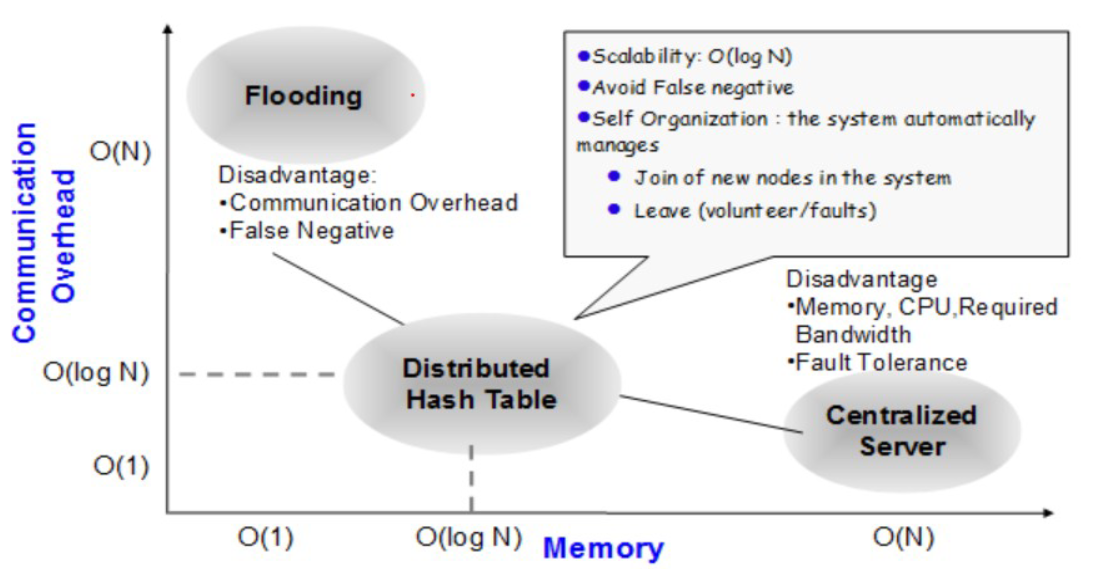
\includegraphics{images/DHT_motivations.png}
   \caption{DHT Motivations}
   \label{fig:DHT_motivations}
\end{figure}

The key idea is to split the hash tables into several parts and distribute them to several servers, and to use hash of resources (or of the URLs of resources) as a key to map them to a
dynamically changing set of web caches, but with \ul{each key mapped to single server}; so that
each machine (user) can locally compute which web cache should contain the
required resource, refenced by an URL.\\
This technique is extended to DHT for P2P systems.

However, \ul{\textbf{rehashing} is a problem in dynamic scenarios} if the hashing scheme depends directly on the number of servers:
$99\%$ of keys have to be remapped, resulting in a lot of messages exchange.
\begin{figure}[htbp]
   \centering
   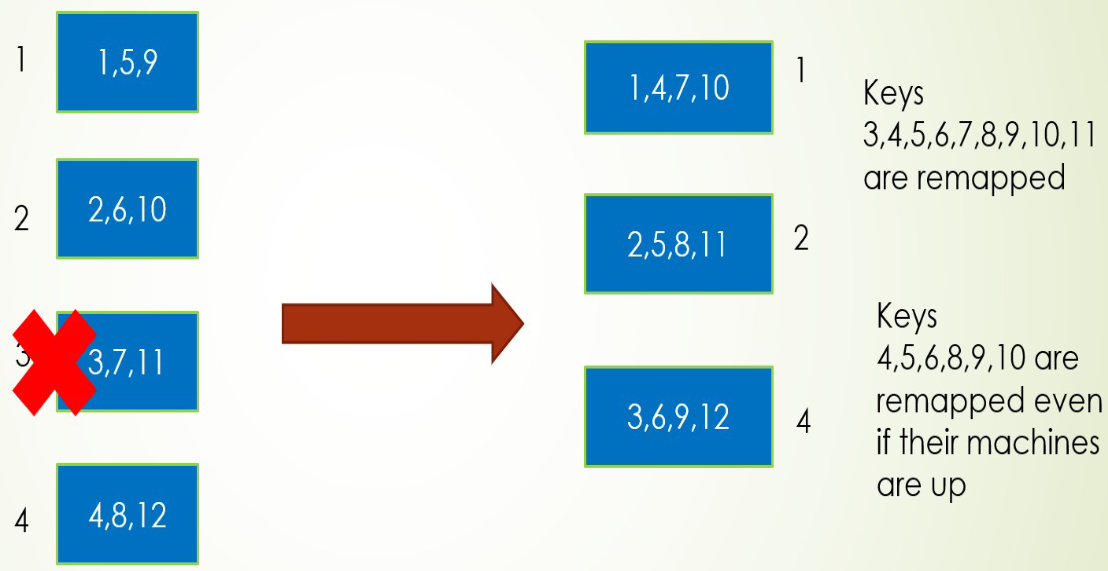
\includegraphics{images/rehashing_problem.png}
   \caption{Rehashing problem}
   \label{fig:rehashing_problem}
\end{figure}

\textbf{Consistent hashing} is a set of hash techniques which guarantees that adding more nodes/remove nodes implies \ul{moving only a minority of data items}.
each node manages ---instead of a set of sparse keys--- an interval of consecutive hash keys, and intervals are joined/splitted when nodes join/leave the network and keys redistributed between adjacent peers.


\begin{paracol}{2}
   % \colfill
   \ul{But how to build DHTs?}
   \begin{itemize}
      \item use a logical name space, called \textit{identifier space} consisting of identifiers
      $\{0,1,2,...,N-1\}$
      \item define identifier space as a \textit{logical ring} modulo $N$
      \item every node picks a random identifier
      through Hash $H$.
   \end{itemize}
   \begin{figure}[htbp]
      \centering
      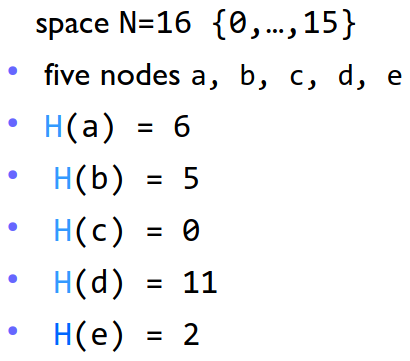
\includegraphics{images/DHT_build2.png}
      % \caption{}
      \label{fig:DHT_build2}
   \end{figure}

   % \colfill
   \switchcolumn
   
   % \begin{adjustbox}{valign=\fill}
   \begin{figure}[htbp]
      \centering
      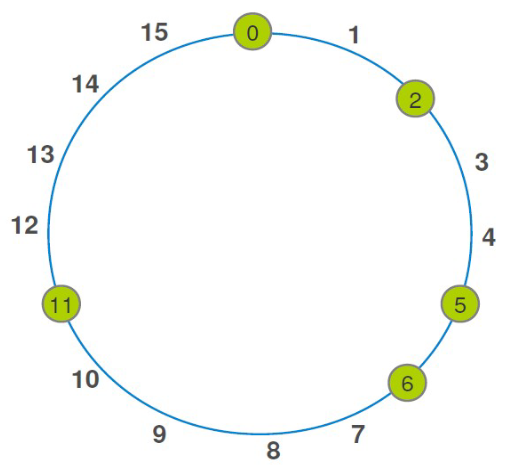
\includegraphics{images/DHT_build1.png}
      \caption{Identifier space}
      \label{fig:DHT_build1}
   \end{figure}
   % \end{adjustbox}
   
\end{paracol}
